\cleardoublepage

\chapter{}
\label{chap:b}

\begin{description}[leftmargin=!,labelwidth=\widthof{\bfseries Volume and number}]
    \item[Title] Machine learning-assisted antenna modelling for realistic assessment of incident power density on non-planar surfaces above 6 GHz
    \item[Authors] Ante Kapetanović, Dragan Poljak
    \item[Journal] Radiation Protection Dosimetry
    \item[Year] 2023
    \item[Volume and number] 199, 8--9
    \item[Pages] 826--834
    \item[Categorization] Research paper
    \item[Language] English
    \item[Abstract] In this paper, the analysis of exposure reference levels is performed for the case of a half-wavelength dipole antenna positioned in the immediate vicinity of non-planar body parts.
    The incident power density (IPD) spatially averaged over the spherical and cylindrical surface is computed at the 6–90 GHz range, and subsequently placed in the context of the current international guidelines and standards for limiting exposure to electromagnetic (EM) fields which are defined considering planar computational tissue models.
    As numerical errors are ubiquitous at such high frequencies, the spatial resolution of EM models needs to be increased which in turn results in increased computational complexity and memory requirements.
    To alleviate this issue, we hybridise machine learning and traditional scientific computing approaches through differentiable programming paradigm.
    Findings demonstrate a strong positive effect the curvature of non-planar models has on the spatially averaged IPD with up to 15\% larger values compared to the corresponding planar model in considered exposure scenarios.
    \item[Databases] Scopus, Google Scholar, Web of Science Core Collection -- Science Citation Index Expanded
    \item[Impact factor] 1.053
    \item[DOI] \href{https://doi.org/10.1093/rpd/ncad114}{\url{10.1093/rpd/ncad114}}
    \item[Copyright notice] \copyright 2023 Oxford University Press. Reprinted, with permission, from Ante Kapetanović and Dragan Poljak, Machine learning-assisted antenna modelling for realistic assessment of incident power density on non-planar surfaces above 6 GHz, Radiation Protection Dosimetry, 2023
\end{description}

\cleardoublepage

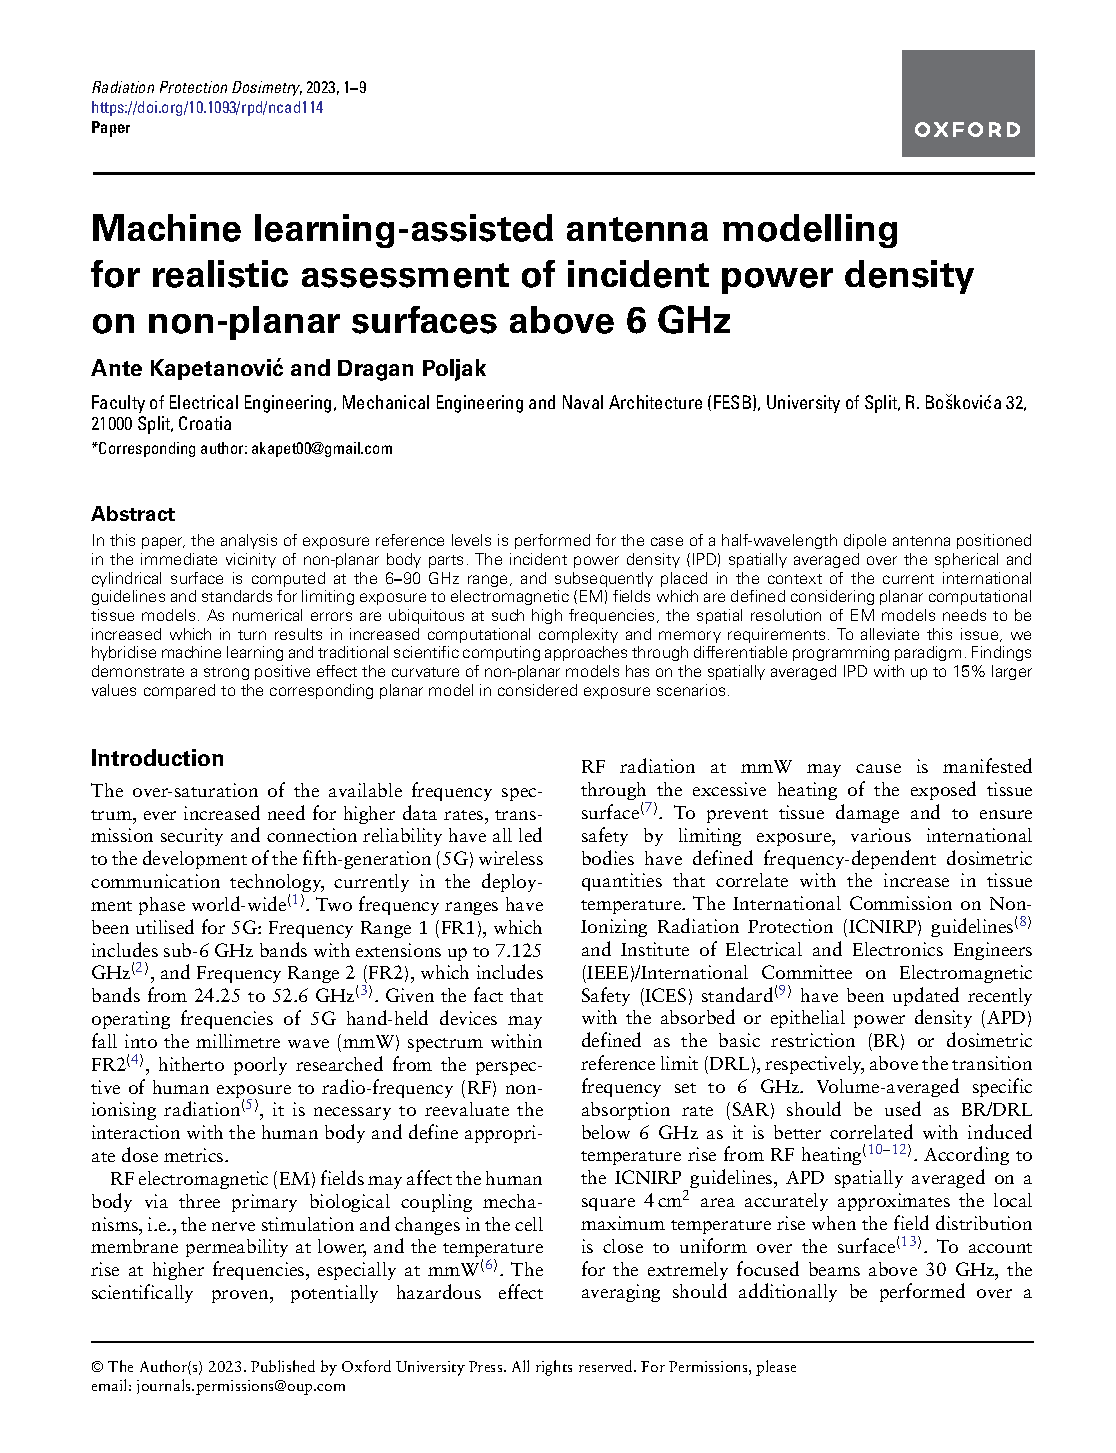
\includepdf[pages=-, pagecommand={\thispagestyle{includepdfstyle}}]{papers/Kapetanovic2023rpd.pdf}
